\chapter{Kubernetes}
\label{chp:kubernetes}

Kubernetes is a production-grade open-source container orchestrator, originally designed by Google.
%
It was soon established as a de-facto standard for automated management, deployment, scaling and CI/CD of containerized micro-service applications in large clusters.
%
%
%Basically, it runs containers on a cluster abstracted as a transparent pool of resources, so as to optimize resources usage and to scale and update containers with no down-time.
%
We choose Kubernetes as the container orchestrator on which to conduct our experiments because 
(i) it is an industrial standard,
(ii) it is portable, extensible and autonomic,
(iii) it is designed for long-running micro-services applications,
(iv) it is based on a innovative deployment schema (Pods)
(iv) it is open-source,
(vi) it is well documented,
(vii) it is supported by an active community.

In this Chapter, we give an overview of Kubernetes as our reference platform to implement and experiment smart elasticity.
%
In particular, we introduce it with a bit of its history, then focus on its main features, architecture, objects and the way it provides elasticity.


% %
% HISTORY
% %
\section{History}
\label{sec:kuberetes-history}
The name Kubernetes originates from the Greek word $\kappa\upsilon\beta\epsilon\rho\nu\epsilon\tau\epsilon\sigma$, that means \textit{helmsman} and is also the etymological root of the term cybernetic\footnote{term coined in 1948 by U.S. mathematician Norbert Wiener (\cite{masani2012norbert}).}.
%
Kubernetes is often refer to as \textit{K8s}, derived by replacing the 8 letters "ubernete" with "8".

Kubernetes was originally designed by Google as the open-source declination of Omega (\cite{burns2016borg}), that is the closed-source containers orchestrator internally used by Google to manage its two billions running containers (\cite{schwarzkopf2013omega}).
%
Kubernetes builds upon over a decade of experience that Google has with running production workloads at scale, combined with best-of-breed ideas and practices from the community (\cite{verma2015large}).
%
The first release was announced on June 2014 with a blog post on \cite{google-announces-kubernetes} and became soon available to the public through the Google Container Engine (\cite{google-container-engine-web}).
%
In 2015, it was donated to the Cloud Native Computing Foundation (\cite{techcrunch-kubernetes-cncf}), a department of the Linux Foundation (\cite{linux-foundation-web}) (the world's largest open source non-profit organization) founded by world's leading tech companies such as Google, IBM and VMWare to promote containers (\cite{zdnet-cncf}).
%
The explosion in popularity of containerization has heavily impacted the development and adoption of Kubernetes.


% %
% FEATURES
% %
\section{Features}
\label{Sec:features}

Kubernetes coordinates a highly available cluster of VMs or physical machines to work together as a single unit. 
%
It provides abstractions that allow to deploy containerized applications to a cluster without hard-wiring them to individual nodes.
%
Hence it realizes a truly \textit{container-centric environment}, opposed to the traditional host-centric infrastructure, which provides the full advantages and benefits inherent to containers.

Kubernetes allows the cluster manager to effectively automate applications delivery to customers by 
(i) deploying containerized applications quickly and predictably,
(ii) scaling applications on the fly,
(iii) rolling out new features with no downtime and
(iv) optimizing resource usage by limiting it to required resources only.

%Kubernetes is 
%(i) \textit{portable}, as it supports both public, private, hybrid and multi-cloud
%(ii) \textit{general purpose}, as it supports both stateless/stateful, micro-service/monoliths and service/batch applications,
%(iii) \textit{extensible}, as it is modular, pluggable, hookable and composable, and
%(iv) \textit{autonomic}, as it provides self-healing functionalities, such as auto-restart, auto-placement and auto-scaling.

The Kubernetes project has been always committed to the following design pillars:

\begin{itemize}
	
	\item \textbf{Portability:} supports both public cloud, private cloud, bare metal and laptop with consistent behavior so that applications and tools are portable throughout the ecosystem.
	
	\item \textbf{Generality:} it is agnostic to applications, as it runs applications that are both stateless and stateful, microservices and monoliths, services and batch, and so on.
	
	\item \textbf{Meet users partway} although it focuses on deployment and management of microservices and cloud-native applications, it provides some mechanisms to facilitate migration of monolithic and legacy applications.
	
	\item \textbf{Flexibility} its functionalities can be consumed a la carte and (in most cases) Kubernetes does not prevent from using custom solutions in lieu of built-in functionalities.
	
	\item \textbf{Extensibility} Kubernetes enables you to integrate it into your environment and to add the additional capabilities you need, by exposing the same interfaces used by built-in functionalities.
	
	\item \textbf{Automation} it dramatically reduce the burden of manual operations. It supports both declarative and imperative control to support higher-level orchestration and automation. The declarative approach is key to the system’s autonomic capabilities.
	
	\item \textbf{CI/CD} users expect applications to be available all the time and developers are expected to deploy new versions frequently.
	%
	Kubernetes provides a mechanism to rool-out/roll-back containers with zero downtime by incrementally updating application instances with new ones and load-balancing the traffic only to available Pods during the update.
	
	\item \textbf{Advance the state of the art} although it intends to support non-cloud-native applications, it aims to drive and advance the cloud-native and DevOps state of the art.
	
\end{itemize}



% %
% ARCHITECTURE
% %
\section{Architecture}
\label{sec:kubernetes-architecture}

Kubernetes follows a master-worker distributed architecture, as depicted in Figure \ref{fig:kubernetes-architecture}.
%
A production Kubernetes cluster should have a minimum of three nodes, one serving as a Kubernetes Master and two serving as Kubernetes Workers.

The \textbf{Kubernetes Master} is responsible for managing the cluster, coordinating all activities, such as scheduling applications, defining and maintaining their desired state, scaling them, and rolling out new updates.
%
The master controls each node so that it is rare to interact with workers directly.
%
The master can be run on a single node, or can be replicated in order to support high-availability clusters.
%
The Master executes the following processes:
%
\begin{itemize}
	
	\item \textbf{API Server:} a web server that exposes a RESTful API to let the user interact with the master to manage the whole cluster.
	%
	Basically, it provides the front-end to the cluster’s shared state through which all other components interact with.
	%
	For example, it allows the user to configure the cluster, check up its state, create, update and delete Kubernetes Objects.
	%
	The \texttt{kubectl} utility is the most convenient way to instruct the server because it encapsulates REST calls into simple and intuitive terminal commands.
	
	\item \textbf{Controller Manager:} a daemon that coordinates all core controllers.
	%
	Each controller watches a portion of the shared state of the cluster and makes changes to drive the actual state towards the desired state.
	%
	These functions have been split into separate components to make them more easily replaceable and extendable.	
	
	\item \textbf{Scheduler:} a policy-rich and topology-aware daemon that determines how to schedule and place containerized applications on Workers.
	%
	To determine the best fit it takes into account a lot of factors, such as resources utilization, quality of service requirements, hardware/software/policy constraints, affinity and anti-affinity specifications, data locality and son on.
	%
	%Kubernetes supports user-provided schedulers and multiple concurrent cluster schedulers, using the shared-state approach pioneered by Omega.
	
	\item \textbf{ETCD:} a distributed reliable key-value database, used to store cluster's state and configurations\footnote{the name \textit{ETCD} is inspired by the Unix system folder \textit{etc}, used to store system configurations, to which the letter \textit{d} has been added with the meaning of \textit{distributed}.} in JSON or Protobuf format.
	%
	It provides a way to store configuration data reliably and to coordinate components by meant of cluster's state changes and can be inspected using the \textit{etcdctl} tool.
	
\end{itemize}

A \textbf{Kubernetes Worker} is responsible for the execution of Pods and to notify local resource state to the Master.
%
Each Worker executes the following processes:
%
\begin{itemize}
	
	\item \textbf{Kubelet:} the primary agent responsible for communication between the Kubernetes Master and the Node and the management of all Pods scheduled on its Node.
	%
	The kubelet works in terms of a \textit{PodSpec}, that is a YAML or JSON that describes a Pod.
	%
	The kubelet takes a set of PodSpecs that are provided through various mechanisms (primarily through the apiserver) and ensures that the containers described in those PodSpecs are running and healthy.
	
	\item \textbf{Container Runtime:} a runtime environment responsible for managing images and running containers.
	%
	Future versions will be provided with a Container Runtime Interface to decouple scheduling operations from the underlying control of containers in order to facilitate pluggability of the container runtime.
	%
	The current version supports Docker (\cite{docker-web}), Rkt (\cite{rkt-web}), Cri-o (\cite{crio-web}), and Frakti (\cite{frakti-web}).
	
	\item \textbf{Proxy:} a daemon responsible for routing requests submitted to Service external IP to the internal virtual IP of the attached back-ends, in a highly-available and load balanced fashion.
	%
	When a user creates a new Service, new rules are added to this component.
	
	\item \textbf{cAdvisor:} a daemon that collects, aggregates and exports performance metrics about containers running on the Node.
	%
	It natively supports Docker containers but future versions are going to support any other container type out of the box.
	
\end{itemize}

Furthermore, a Kubernetes cluster is provided with \textbf{Cluster Add-Ons}, that are built-in Deployments and Services considered an inherent part of a Kubernetes cluster.
%
The most notable addons are \textit{GUI}, providing a convenient web interface to interact with the cluster, and \textit{Heapster}, providing monitoring service about performance statistics for the whole cluster.
%
For a complete list of such add-ons, we refer the reader to \cite{kubernetes-web}.

The Kubernetes architecture is often partitioned into
(i) the \textbf{Control Plane}, constituted by the Kubernetes Master and Kubelet, responsible to make the cluster’s current state match the desired state.
(ii) the \textbf{Execution Plane}, constitute by Container Runtime, Proxy, cAdvisor and add.ons, responsible for the real execution of containers.

\begin{figure}	
	\label{fig:kubernetes-cluster}
	\centering
	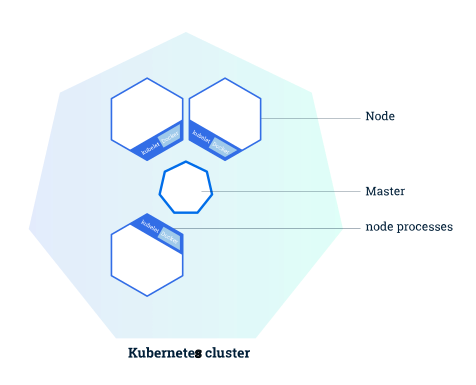
\includegraphics[width=.7\columnwidth]{kubernetes-cluster}
	\caption{Kubernetes cluster.}
\end{figure}

\begin{figure}	
	\label{fig:kubernetes-architecture}
	\centering
	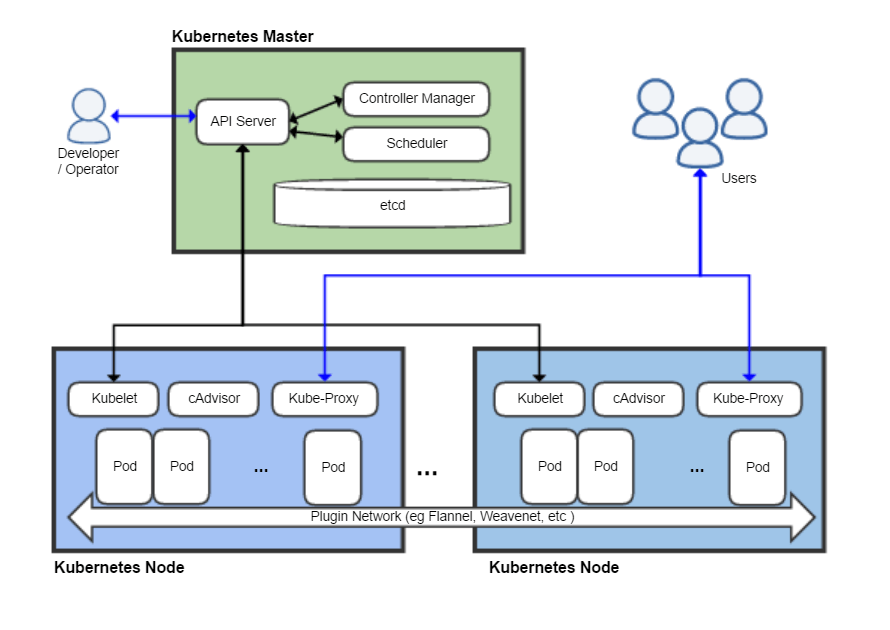
\includegraphics[width=.7\columnwidth]{kubernetes-architecture}
	\caption{Kubernetes architecture.}
\end{figure}


\section{Objects}
\label{sec:kubernetes-objects}
Kubernetes provides some abstractions to represent and manage the state of the cluster.
%
These abstractions are called \textit{Kubernetes Objects} (or simply Objects, for short) and are persistent entities within the Kubernetes system, thus representing the core API building blocks.
%
Each Kubernetes Object characterizes the desired cluster's state, that is why it is sometimes refer to as a "record of intent".
%
Objects are managed, i.e. created updated and deleted, by submitting requests to the Kubernetes REST API.

The main abstractions, at least the ones related to our work, are \textit{Deployment}, \textit{Pod}, \textit{Service} and \textit{HorizontalPodAutoscaler}.
%
We refer the reader to \cite{kubernetes-web} for a complete description of all objects.

A \textbf{Deployment} defines the desired state for an application in a declarative fashion.
%
It defines the state in terms of 
(i) composing containers 
(ii) number of replicas
(iii) constraints of resource utilization
%
The creation of a new Deployment is the creation of a new invariant to satisfy.

A \textbf{Pod} is the smallest deployable unit of computing that can be created and managed in Kubernetes, serving as a unit of deployment, horizontal scaling, and replication.
%
A Pod is a group of one or more containers that are co-scheduled on the same node together with a specification defining how to run them.
%
Containers in a Pod share the same storage (volumes) and network (IP address, port space); furthermore they can easily communicate via IPC primitives.
%
This is why containers that need to work together are usually added to the same Pod.
%
A Pod should be viewed as a cohesive unit of service and it can be made of 
(i) a single container, where a Pod is a simple wrapper around a container or 
(ii) a group of tightly coupled containers forming a single instance of a composite application.
%
For example a Pod can be used to host vertically integrated application stacks, such as LAMP.
%
Like well-designed containers following the micro-services model, well-designed pods should be \textit{focused}, \textit{stateless}, and \textit{concurrent}, as Kubernetes assumes that pods can be deleted, created, and replicated at will.
%
Pod abstraction is convenient because it realizes decoupling of software dependencies thus making easier and more effective the general management and the CI/CD automation.
%
%A Pod's lifecycle is made of the following phases:
%
%\begin{itemize}
%	\item \textbf{Pending:} The API Server has created a pod resource and stored it in etcd, but the pod has not been scheduled yet, nor have container images been pulled from the registry.
%	\item \textbf{Running:} The pod has been scheduled to a node and all containers have been created by the kubelet.
%	\item \textbf{Succeeded:} All containers in the pod have terminated successfully and will not be restarted.
%	\item \textbf{Failed:} All containers in the pod have terminated. At least one container has terminated in failure.
%	\item \textbf{Unknown:} The API Server was unable to query the state of the pod, typically due to an error in communicating with the kubelet.
%\end{itemize}
%
%When you do a kubectl get pod, note that the STATUS column might show a different message than the above five messages, such as Init:0/1 or CrashLoopBackOff. This is due to the fact that the phase is only part of the overall status of a pod.
%
%Not shown in the diagram, before anything else, the infra container is launched establishing namespaces the other containers join.
%The first user-defined container launching is the init container which you can use for pod-wide initialization.
%Next, the main container and the post-start hook launch at the same time, in our case after 4 seconds. You define hooks on a per-container basis.
%Then, at second 7, the liveness and readiness probes kick in, again on a per-container basis.
%At second 11, when the pod is killed, the pre-stop hook is executed and finally, the main container is killed, after a grace period. Note that the actual pod termination is a bit more complicated.
%
%The livenessProbe is used by the kubelet to determine if and when to re-start a container and by a deployment to decide if a rolling update is successful.
%
%The readinessProbe is used by a service to determine if a pod should receive traffic.
%
%\begin{figure}	
%	\label{fig:kubernetes-pod-lifecycle}
%	\centering
%	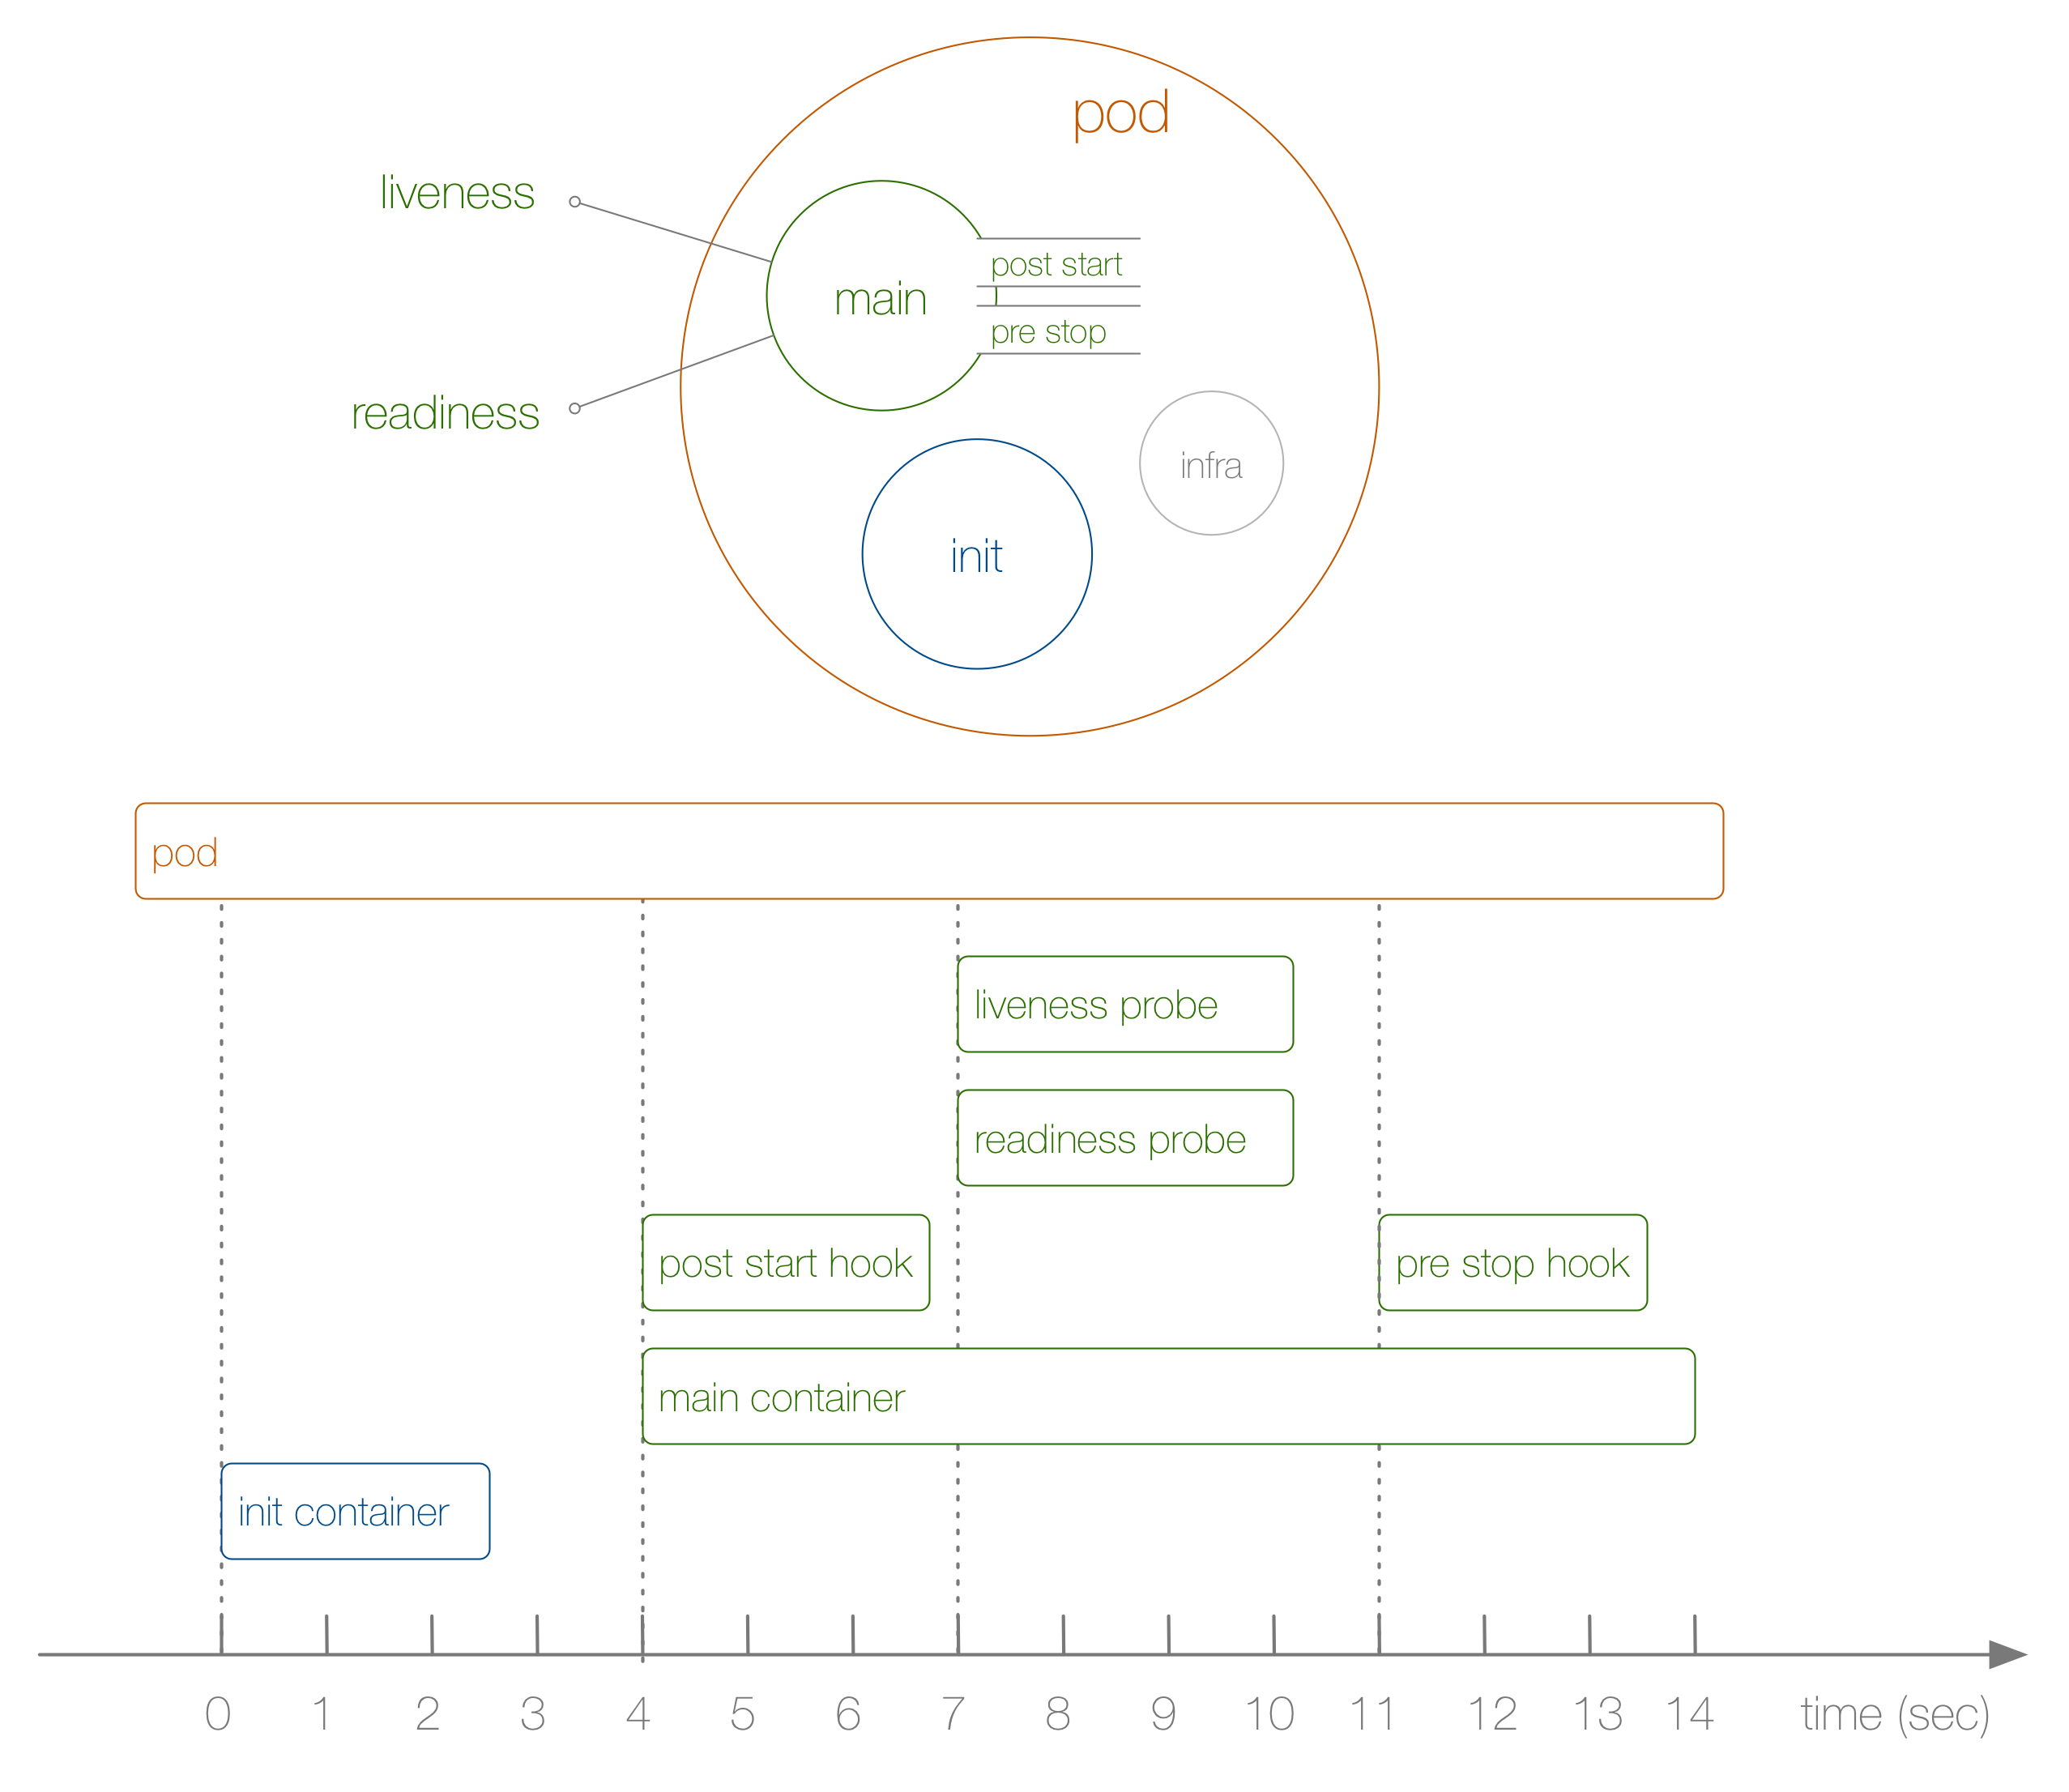
\includegraphics[width=.7\columnwidth]{kubernetes-pod-lifecycle}
%	\caption{Kubernetes Pod lifecycle.}
%\end{figure}

A \textbf{Service} defines single long-running access-point for a logical set of Pods.
%
It allows
(i) load-balanced exposure to external traffic (although each Pod has a unique IP address, those IPs are not exposed outside the cluster without a Service),
(ii) routing across dependent Pods (entities do not communicate with a specific Pod, but with a Service)
(iii) loose coupling between dependent Pods (distinct application services are managed by distinct Service abstractions).
(vi) auto-scaling with no down-time, as the Service ensures lets new replicas dynamically join/exit the set of Pods.

Each object instance can be associated with a collection of \textit{labels}, that are key/value pairs metadata that can be used to classify and filter objects.
%
For example, a Service can be defined to expose only Pods with a specific label, so as to automatically join those Pods once created.

\begin{figure}	
	\label{fig:kubernetes-services}
	\centering
	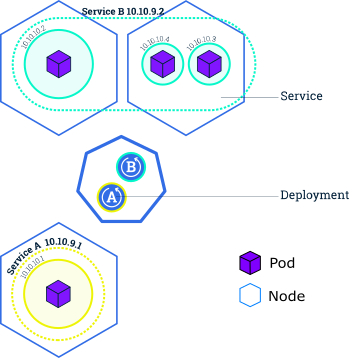
\includegraphics[width=.7\columnwidth]{kubernetes-services}
	\caption{Kubernetes Service deployment.}
\end{figure}

\begin{figure}	
	\label{fig:kubernetes-horizontal-pod-autoscaler}
	\centering
	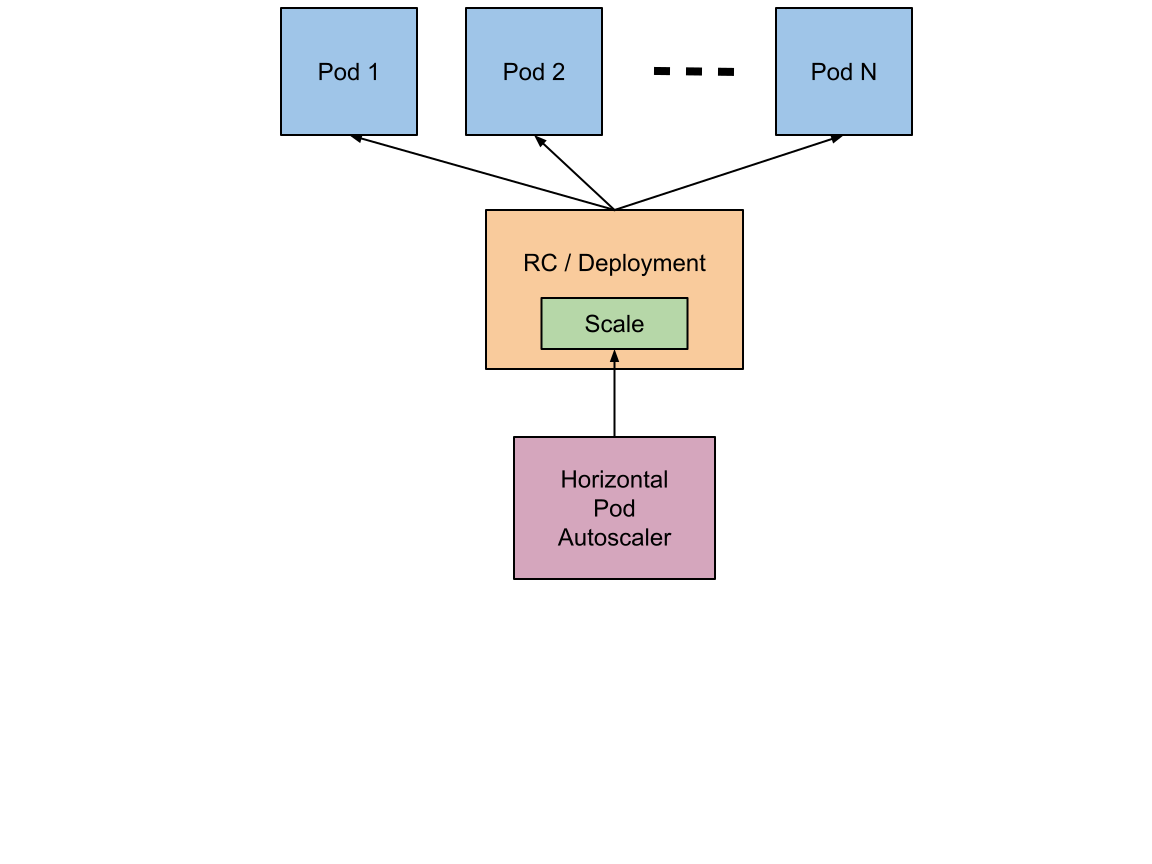
\includegraphics[width=.7\columnwidth]{kubernetes-horizontal-pod-autoscaler}
	\caption{Kubernetes Horizontal Pod Auto-scaler.}
\end{figure}

A \textbf{HorizontalPodAutoscaler} defines the range of resources utilization that each Pod should work in, inducing horizontal scaling actions to satisfy these bounds.
%
We refer the reader to Section \ref{sec:kubernetes-elasticity} for a deep dive into this object and how it realizes elasticity.


% %
% WORKFLOW
% %
%\section{Workflow}
%\label{sec:kubernetes-workflow}
%When you deploy applications on Kubernetes, you tell the master to start the application containers.
%The master schedules the containers to run on the cluster's nodes.
%The nodes communicate with the master using the Kubernetes API, which the master exposes.
%End users can also use the Kubernetes API directly to interact with the cluster.
%we created a Deployment, and then exposed it publicly via a Service.


% %
% API SERVER
% %
%On a conceptual level, Kubernetes is made up of a bunch of nodes with different roles. The control plane on the master node(s) consists of the API Server, the Controller Manager and Scheduler(s). The API Server is the central management entity and the only component that directly talks with the distributed storage component etcd. It provides the following core functionality:

%Serves the Kubernetes API, used cluster-internally by the worker nodes as well as externally by kubectl
%Proxies cluster components such as the Kubernetes UI
%Allows the manipulation of the state of objects, for example pods and services
%Persists the state of objects in a distributed storage (etcd)

%The Kubernetes API is a HTTP API with JSON as its primary serialization schema, however it also supports Protocol Buffers, mainly for cluster-internal communication.

%For extensibility reasons Kubernetes supports multiple API versions at different API paths, such as  /api/v1 or /apis/extensions/v1beta1. Different API versions imply different levels of stability and support:

%Alpha level, for example v1alpha1 is disabled by default, support for a feature may be dropped at any time without notice and should only be used in short-lived testing clusters.
%Beta level, for example v2beta3, is enabled by default, means that the code is well tested but the semantics of objects may change in incompatible ways in a subsequent beta or stable release.
%Stable level, for example, v1 will appear in released software for many subsequent versions.

%In general the Kubernetes API supports create, update, delete, and retrieve operations at the given path via the standard HTTP verbs POST, PUT, DELETE, and GET with JSON as the default payload.

%Let’s now have a look at how the HTTP API space is constructed.
%Most API objects make a distinction between the specification of the desired state of the object and the status of the object at the current time. A specification is a complete description of the desired state and is persisted in stable storage.

%API Group is a collection of Kinds that are logically related. For example, all batch objects like Job or ScheduledJob are in the batch API Group.

%Version. Each API Group can exist in multiple versions. For example, a group first appears as v1alpha1 and is then promoted to v1beta1 and finally graduates to v1. An object created in one version (e.g. v1beta1) can be retrieved in each of the supported versions (for example as v1).

%Resource is the representation of a system entity sent or retrieved as JSON via HTTP; can be exposed as an individual resource (such as .../namespaces/default) or collections of resources (like .../jobs).

%An API Group, a Version and a Resource (GVR) uniquely defines a HTTP path.

%More precisely, the actual path for jobs is /apis/batch/v1/namespaces/$NAMESPACE/jobs because jobs are not a cluster-wide resource, in contrast to, for example, node resources. For brevity, we omit the $NAMESPACE segment of the paths throughout the post.

%Now that we’ve reviewed the terminology used in the Kubernetes API we move on to how API requests are processed. The API lives in k8s.io/pkg/api and handles requests from within the cluster as well as to clients outside of the cluster.

%\begin{figure}	
%	\label{fig:kubernetes-achitecture-2}
%	\centering
%	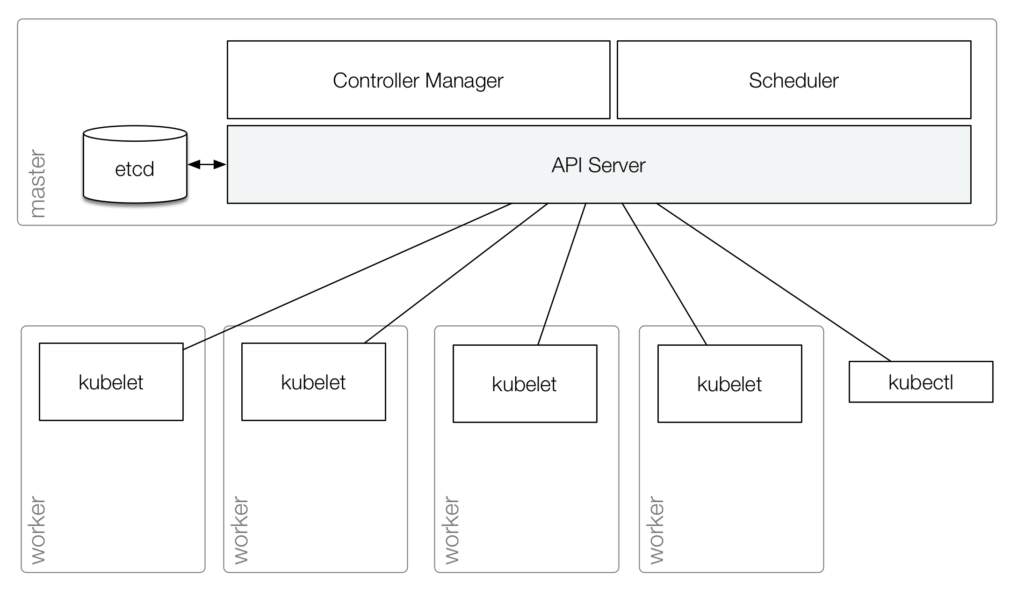
\includegraphics[width=.7\columnwidth]{kubernetes-architecture-2}
%	\caption{Kubernetes architecture 2}
%\end{figure}

%\begin{figure}	
%	\label{fig:kubernetes-apis}
%	\centering
%	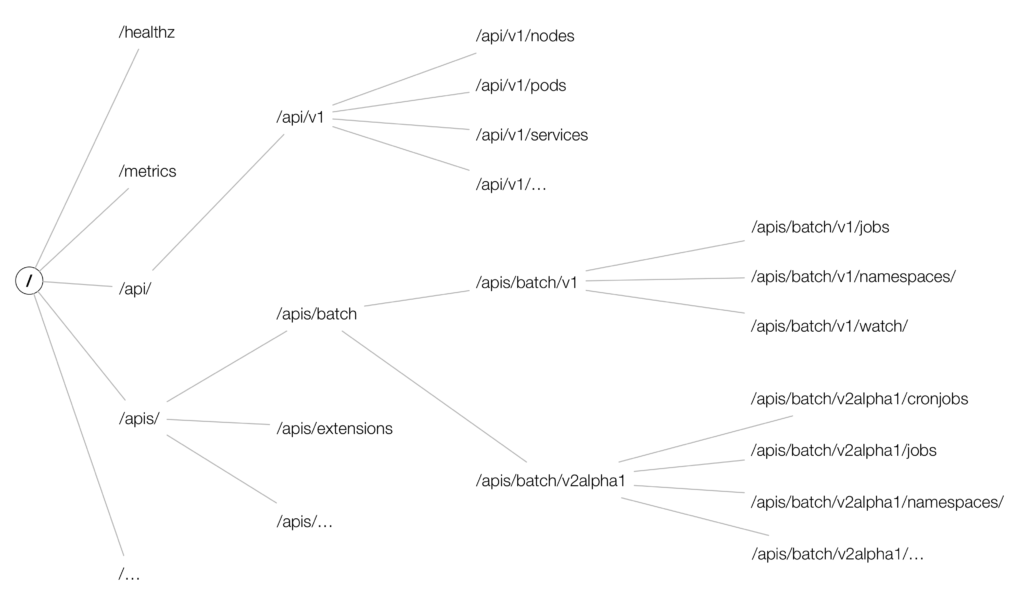
\includegraphics[width=.7\columnwidth]{kubernetes-apis}
%	\caption{Kubernetes APIs}
%\end{figure}

% %
% ELASTICITY
% %
\section{Elasticity}
\label{sec:kubernetes-elasticity}

Kubernetes implements elasticity, following the \textit{reactive threshold-based model} (see Chapter \ref{chp:elasticity}).
%
The elasticity is implemented in a per-Deployment fashion by the \textbf{HorizontalPodAutoscaler (HPA)}, whose operation is depicted in Figure \ref{fig:kubernetes-horizontal-pod-autoscalerorizontal-pod-autoscaler}.
%
The HPA periodically adjusts the replication degree of Pods for a specific Deployment 
\footnote{The replication degree of a Pod is determined by the parameter \texttt{replica} of the Deployment that originates it.}
(default is one replica), such that replicas operate within a target resource utilization range, defined in Deployment declaration.
%
A HPA is created and associated to a specific Deployment by the \texttt{autoscale} command provided by \texttt{kubectl}.
%
For example, running the following command:
%
\begin{verbatim}
kubectl autoscale deployment foo --min=2 --max=100 --cpu-percent=8
\end{verbatim}
%
creates or updates a HPA associated to the deployment \texttt{foo} bounding replicas between 2 and 100 with target CPU utilization equal to 80\%.

Once created, HPA operates as a control loop, with a default period of 30 seconds.
%
On each period it queries Heapster for metrics on targeted Pods at a set interval to determine the current resource utilization of Pods, and performs horizontal auto-scaling actions to preserve the desired level of per replica Pod resource utilization.
%
Initially, the only resource on which it was possible to determine auto-scaling behavior was CPU utilization percentage.
%
Latest versions added support for auto-scaling based on custom metrics such as memory usage.
%
As traffic increases [decreases], the application needs to scale out [in] to keep up with user demand, that is the Deployment replication degree needs to be increased [decreased], in response to the fact that resource utilization increases [decreases].

The current algorithm to adjust the replication degree at each interval of the control loop is fairly simple
\footnote{The auto-scaling algorithm is implemented by the class \textit{kubernetes/pkg/controller/podautoscaler/replica\_calculator.go}}.
%
In particular the replication degree is updated according to the following Equation:
%
\begin{equation}
\label{eqn:kubernetes-auto-scaling}
\rho_{f} = \Biggl\lceil\frac{\sum_{i=1}^{\rho_{i}} \eta_{i}}{\overline{\eta}}\Biggr\rceil
\end{equation}
%
where
$\rho_{f}$ is the final replication degree,
$\rho_{i}$ is the initial replication degree,
$\eta_{i}$ is the utilization for the $i$-th pod and
$\overline{\eta}$ is the target utilization.
%
Note that the ceiling function ensures that no fractions of Pods can be created.
%
The resource utilization is calculated as the average utilization across the last minute, divided by the total resource requested by the Pod. 
%
In Kubernetes version 1.1, CPU usage is taken directly from Heapster. In future, there will be API on master for this purpose.
%
Starting and stopping pods may introduce noise to the metric (for instance, starting may temporarily increase CPU). So, after each action, the autoscaler should wait some time for reliable data. Scale-up can only happen if there was no rescaling within the last 3 minutes. Scale-down will wait for 5 minutes from the last rescaling.
%
Such approach has two benefits: 

(i) \textit{conservative auto-scaling}, that is giving more priority to rapidly increase replicas rather than decreasing them in response to load changes.

(ii) \textit{trashing avoidance}, that is to prevent rapid execution of conflicting decision if the load is not stable.

\begin{figure}	
	\label{fig:kubernetes-scaling-1}
	\centering
	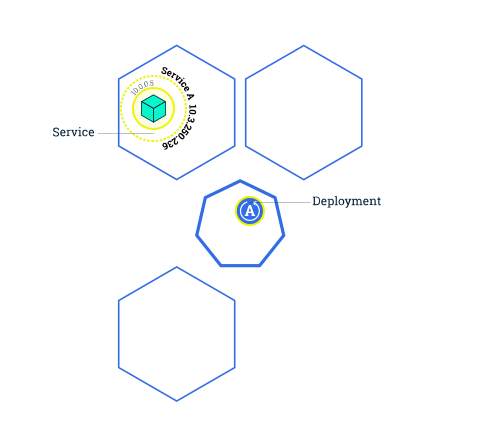
\includegraphics[width=.7\columnwidth]{kubernetes-scaling-1}
	\caption{Kubernetes scaling: not scaled.}
\end{figure}

\begin{figure}	
	\label{fig:kubernetes-scaling-2}
	\centering
	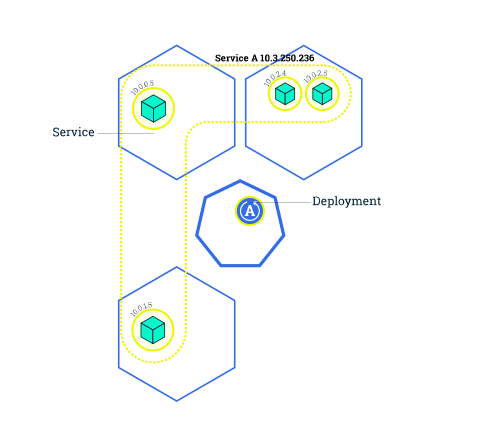
\includegraphics[width=.7\columnwidth]{kubernetes-scaling-2}
	\caption{Kubernetes scaling: scaled.}
\end{figure}

To keep auto-scaling from being overly \textit{sensitive}, scaling will only occur if the current resource utilization is outside of a 10\% tolerance range.
%
To keep auto-scaling from being overly \textit{frequent}, once a scale up or scale down happens, no more auto-scaling will occur for a constant threshold interval $T_{wait}$.
%
This waiting time prevents \textit{thrashing} by ensuring auto-scaling can actually take effect before it is potentially attempted again.
%
By default, this interval is set to five minutes from the most recent down-scaling and three minutes from the most recent up-scaling. 
%
Notice that up-scaling is given a greater priority than down-scaling.

Finally notice that, although not yet implemented, Kubernetes reliance upon containers means vertical auto-scaling is a possibility in the near future, as there are a variety of methods for increasing the resources available to a container without stopping execution (\cite{matthias2015docker}).

For a more complete and general coverage about how auto-scaling works, we refer the reader to the official design documents in \cite{kubernetes-hpa-design-web}.


\section{Extensions}
\label{sec:kubernetes-extensions}

Initially, the only way to extend Kubernetes's core was to fork and patch the source code.
%
This initial approach is affected by evident drawbacks due to lack of portability.
%
To let the core be both flexible and light, the project came up with two ways to extend it: Custom Resource Definition and User API Server.

A \textbf{Custom Resource Definition (CRD)} is a YAML file to define a Custom Resource (CR), that is a custom object whose lifecycle is managed by Kubernetes in the same way built-in objects are.
%
Custom objects extends the Kubernetes API allowing to introduce custom APIs.
%
When a CRD is submitted to the API Server, Kubernetes reacts by creating a new CRD and an associated RESTful resource path to manage its CR.
%
Once CRD has been created, CRs can be managed in a way that is indistinguishable with respect to native objects from the user point of view. For exampe, they can be managed both via kubectl, REST APIs and the Web Dashboard.
%
This is the easiest way to extend core objects, as it requires only to submit to the API Server an object definition expressed as a YAML specification.
%
Figure \ref{fig:kubernetes-crd} shows an example of a CRD which creates the RESTful resource path \textit{/apis/stable.example.com/v1/namespaces/*/databases}.

\begin{figure}
\label{fig:kubernetes-crd}
\lstinputlisting{code/kubernetes-crd.yaml}
\caption{Custom Resource Definition for the database object.}
\end{figure}
%
%Custom objects support finalizers, which allow controllers to implement conditions that must be completed before the object can be deleted. The first delete request on an object with finalizers sets a value for the metadata.deletionTimestamp field instead of deleting the object. This triggers controllers watching the object to execute any finalizers they handle. Each controller then removes the finalizer from the list and issues the delete request again. This request deletes the object only if the list of finalizers is empty, meaning all finalizers are done.

\textbf{User API Servers (UAS)} is a custom API server that realizes a controller and related resources, running in parallel to the Kubernetes API Server.
This is the most flexible way to define custom controllers and custom resources as it provides the most fine-grained control over what is going on with resources and their overall lifecyle.

A UAS is deployed as a containerized application launched within the cluster. 
%
A UAS is nothing more than a Go, Python or Java application that interacts with Kubernetes's controller manager by the Kubernetes Client API.
%
Figure \ref{fig_kubernetes-uas} shows an example of how a UAS works.
%
We refer the reader to Chapter \ref{chp:implementation} for a detailed description about how a UAS can be developed.

\begin{figure}	
	\label{fig:kubernetes-uas}
	\centering
	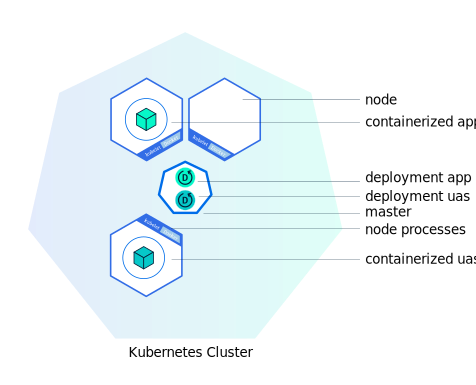
\includegraphics[width=.7\columnwidth]{kubernetes-uas}
	\caption{Kubernetes User API Server}
\end{figure}


% %
% METRICS API
% %
\section{Metrics}
\label{sec:kubernetes-metrics}
Understanding how an application behaves when deployed is crucial to scaling the application and providing a reliable service. In a Kubernetes cluster, application performance can be examined at many different levels: containers, pods, services, and whole clusters. As part of Kubernetes we want to provide users with detailed resource usage information about their running applications at all these levels. This will give users deep insights into how their applications are performing and where possible application bottlenecks may be found. In comes Heapster, a project meant to provide a base monitoring platform on Kubernetes.

Heapster is a cluster-wide aggregator of monitoring and event data. It currently supports Kubernetes natively and works on all Kubernetes setups. Heapster runs as a pod in the cluster, similar to how any Kubernetes application would run. The Heapster pod discovers all nodes in the cluster and queries usage information from the nodes’ Kubelets, the on-machine Kubernetes agent. The Kubelet itself fetches the data from cAdvisor. Heapster groups the information by pod along with the relevant labels. This data is then pushed to a configurable backend for storage and visualization. Currently supported backends include InfluxDB (with Grafana for visualization), Google Cloud Monitoring and many others described in more details here. The overall architecture of the service can be seen below:

\begin{figure}	
	\label{fig:kubernetes-monitoring-architecture}
	\centering
	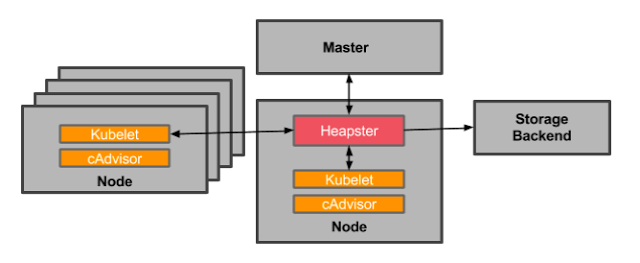
\includegraphics[width=.7\columnwidth]{kubernetes-monitoring-architecture}
	\caption{Kubernetes monitoring architecture leveraging Heapster.}
\end{figure}

cAdvisor is an open source container resource usage and performance analysis agent. It is purpose-built for containers and supports Docker containers natively. In Kubernetes, cAdvisor is integrated into the Kubelet binary. cAdvisor auto-discovers all containers in the machine and collects CPU, memory, filesystem, and network usage statistics. cAdvisor also provides the overall machine usage by analyzing the ‘root’ container on the machine.

On most Kubernetes clusters, cAdvisor exposes a simple UI for on-machine containers on port 4194. Here is a snapshot of part of cAdvisor’s UI that shows the overall machine usage:

%\begin{figure}	
%	\label{fig:kubernetes-cadvisor-ui}
%	\centering
%	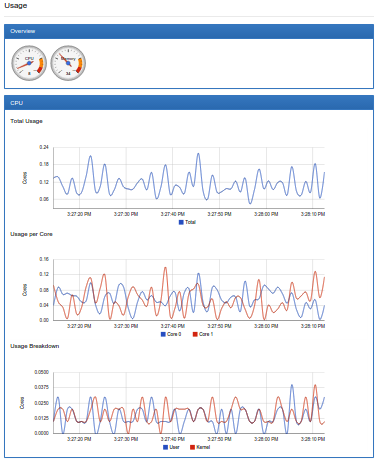
\includegraphics[width=.7\columnwidth]{kubernetes-cadvisor-ui}
%	\caption{Interfaces of cAdvisor.}
%\end{figure}

A Grafana setup with InfluxDB is a very popular combination for monitoring in the open source world. InfluxDB exposes an easy to use API to write and fetch time series data. Heapster is setup to use this storage backend by default on most Kubernetes clusters. A detailed setup guide can be found here. InfluxDB and Grafana run in Pods. The pod exposes itself as a Kubernetes service which is how Heapster discovers it.

The Grafana container serves Grafana’s UI which provides an easy to configure dashboard interface. The default dashboard for Kubernetes contains an example dashboard that monitors resource usage of the cluster and the pods inside of it. This dashboard can easily be customized and expanded. Take a look at the storage schema for InfluxDB here.

%\begin{figure}	
%	\label{fig:kubernetes-heapster-ui}
%	\centering
%	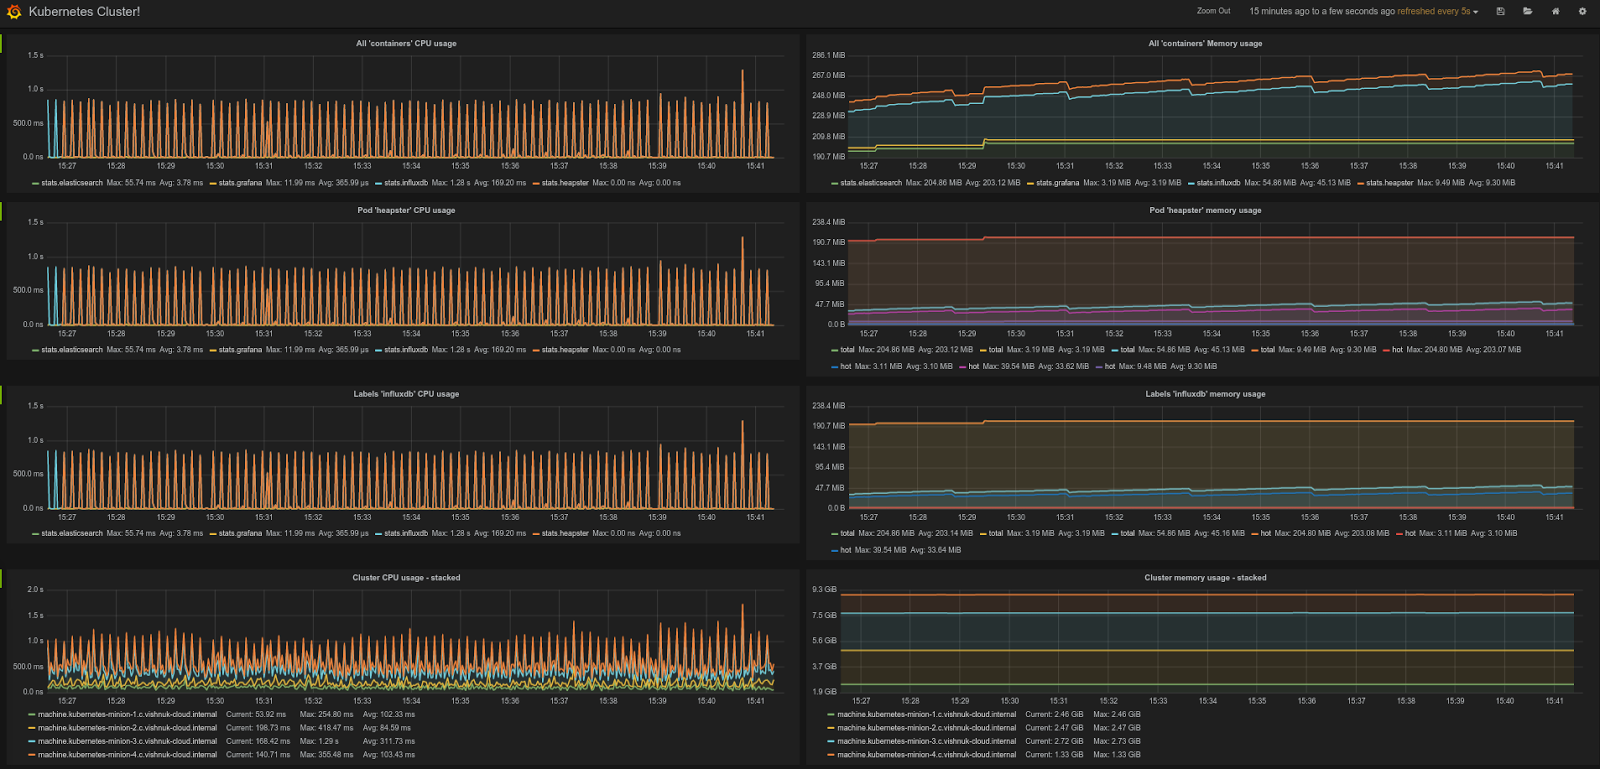
\includegraphics[width=.7\columnwidth]{kubernetes-heapster-ui}
%	\caption{Interfaces of Heapster leveraging Grafana.}
%\end{figure}

Starting from Kubernetes 1.8, resource usage metrics, such as container CPU and memory usage, are available in Kubernetes through the Metrics API. These metrics can be either accessed directly by user, for example by using kubectl top command, or used by a controller in the cluster, e.g. Horizontal Pod Autoscaler, to make decisions.

Through the Metrics API you can get the amount of resource currently used by a given node or a given pod. This API doesn’t store the metric values, so it’s not possible for example to get the amount of resources used by a given node 10 minutes ago.

The API no different from any other API:

it is discoverable through the same endpoint as the other Kubernetes APIs under /apis/metrics.k8s.io/ path
it offers the same security, scalability and reliability guarantees
The API is defined in k8s.io/metrics repository. You can find more information about the API there.

Note: The API requires metrics server to be deployed in the cluster. Otherwise it will be not available.

Metrics Server is a cluster-wide aggregator of resource usage data. Starting from Kubernetes 1.8 it’s deployed by default in clusters created by kube-up.sh script as a Deployment object. If you use a different Kubernetes setup mechanism you can deploy it using the provided deployment yamls. It’s supported in Kubernetes 1.7+ (see details below).

Metric server collects metrics from the Summary API, exposed by Kubelet on each node.

Metrics Server registered in the main API server through Kubernetes aggregator, which was introduced in Kubernetes 1.7.

Learn more about the metrics server in the design doc.